\documentclass[11pt]{report}
\usepackage[utf8]{inputenc}
\usepackage{babel}
\babelprovide[main,import]{spanish}
\usepackage{amsmath,amssymb,amsthm}
\usepackage{geometry}
\geometry{margin=2.5cm}
\usepackage{setspace}
\onehalfspacing
\usepackage{booktabs}
\usepackage{tikz}
\usepackage{pgfplots}
\pgfplotsset{compat=1.18}
\usepgfplotslibrary{groupplots}
\usepackage{hyperref}

\renewcommand{\thesection}{\arabic{section}}
\newtheorem{resultado}{Resultado}

\newcommand{\ket}[1]{\left|#1\right\rangle}
\newcommand{\bra}[1]{\left\langle#1\right|}
\newcommand{\spl}{\sigma_{+}}
\newcommand{\smi}{\sigma_{-}}
\newcommand{\GG}{\Gamma_{2}}
\newcommand{\Lv}{\mathcal{L}}

\title{Brecha de Liouville de un oscilador con intercambio de pares\\ mediado por un sistema de dos niveles con p\'erdida:\\ soluci\'on exacta, punto excepcional y techo $\kappa/4$}
\author{Jhon Sebasti\'an Garc\'ia Barrera}
\date{Septiembre de 2026}

\begin{document}
\maketitle

\begin{abstract}
Se deriva paso a paso la brecha de Liouville del modelo m\'inimo que describe el esquema de Naseem en el r\'egimen resonante: un oscilador acoplado a un sistema de dos niveles con p\'erdida mediante el intercambio de pares $G[(a^{2}-\alpha^{2})\sigma_{+}+\mathrm{h.c.}]$. Para $\alpha=0$ el problema es exactamente soluble: el Liouvilliano es triangular por bloques, sus autovalores se obtienen de un Hamiltoniano no herm\'itico de $2\times 2$ y la brecha tiene la forma cerrada $\Delta=(\kappa/4)[1-\sqrt{1-8\Gamma_{2}/\kappa}]$ hasta un punto excepcional en $\Gamma_{2}=\kappa/8$, a partir del cual queda fija en $\kappa/4$. Para $\alpha\neq 0$ se deriva el l\'imite adiab\'atico, se da un argumento f\'isico del techo $\kappa/4$ y se verifica todo num\'ericamente. El resultado central es negativo para la hip\'otesis previa: el modelo m\'inimo explica la saturaci\'on pero no produce un m\'aximo seguido de un descenso. El m\'aximo observado en el modelo completo requiere otros ingredientes.
\end{abstract}

\section{Planteamiento del problema}

\subsection{Motivaci\'on}

En las simulaciones de Floquet del modelo completo de Naseem \cite{Naseem2026} se observ\'o que la brecha de confinamiento, es decir, la tasa de relajaci\'on m\'as lenta hacia el espacio de los gatos, no crece indefinidamente con el acoplamiento efectivo, como predice la ecuaci\'on maestra adiab\'atica. En cambio, satura en valores del orden de $0.10\kappa$ a $0.17\kappa$ y presenta un m\'aximo cerca de $\Gamma_{2}^{-}/\kappa\approx 0.13$. Se propuso como hip\'otesis que ese m\'aximo es un punto excepcional del intercambio entre el qubit y los pares de fonones, con condici\'on $g_{\mathrm{eff}}\sqrt{n(n-1)}=\kappa/4$. El objetivo de este documento es derivar la brecha de forma expl\'icita y decidir si la hip\'otesis se sostiene.

\subsection{Modelo m\'inimo}

Tras la transformaci\'on polar\'onica y en el marco rotante resonante ($\omega_{q}=2\omega_{m}$), la parte del Hamiltoniano de Naseem responsable del confinamiento es el intercambio de pares con el qubit. Se considera el modelo m\'inimo
\begin{equation}
H = G\left[(a^{2}-\alpha^{2})\,\spl + (a^{\dagger 2}-\alpha^{2})\,\smi\right],
\label{eq:H}
\end{equation}
donde $a$ es el operador de aniquilaci\'on del modo mec\'anico, $\spl=\ket{e}\bra{g}$ y $\smi=\ket{g}\bra{e}$ son los operadores del qubit, $G$ es el acoplamiento efectivo de pares (en la notaci\'on de la tesis, $G=g_{\mathrm{eff}}=2g$) y $\alpha^{2}$ es real y fijado por el drive. El qubit decae con tasa $\kappa$, de modo que la ecuaci\'on maestra es
\begin{equation}
\dot\rho = \Lv\rho = -i[H,\rho] + \kappa\left(\smi\rho\spl - \tfrac{1}{2}\{\spl\smi,\rho\}\right).
\label{eq:ME}
\end{equation}
Se omiten deliberadamente la p\'erdida de un fon\'on, los canales $\Gamma_{1}^{\pm}$, el Kerr, el desplazamiento de Lamb y la desinton\'ia del qubit. La idea es aislar el mecanismo del intercambio de pares y ver si por s\'i solo produce el m\'aximo.

Se define la tasa de disipaci\'on de pares adiab\'atica
\begin{equation}
\GG \equiv \frac{4G^{2}}{\kappa},
\label{eq:G2}
\end{equation}
que coincide con la definici\'on $\Gamma_{2}^{-}=4g_{\mathrm{eff}}^{2}/\kappa$ usada en las tareas num\'ericas. Todas las tasas se expresan en unidades de $\kappa$.

\subsection{Definici\'on de la brecha}

El Liouvilliano $\Lv$ es un superoperador lineal. Sus autovalores $\lambda_{k}$ cumplen $\mathrm{Re}\,\lambda_{k}\leq 0$. Los autovalores nulos corresponden al espacio estacionario. Se define la brecha como
\begin{equation}
\Delta \equiv \min_{k:\,\lambda_{k}\neq 0}\left|\mathrm{Re}\,\lambda_{k}\right|,
\end{equation}
es decir, la tasa del modo no estacionario m\'as lento. Es la tasa a la que un estado perturbado regresa al espacio estacionario.

\subsection{Reescritura con Hamiltoniano no herm\'itico}

Desarrollando el anticonmutador en la Ec.~\eqref{eq:ME},
\begin{align}
\Lv\rho &= -iH\rho + i\rho H - \frac{\kappa}{2}\spl\smi\rho - \frac{\kappa}{2}\rho\spl\smi + \kappa\smi\rho\spl\\
&= -i\left(H - \frac{i\kappa}{2}\spl\smi\right)\rho + i\rho\left(H + \frac{i\kappa}{2}\spl\smi\right) + \kappa\smi\rho\spl.
\end{align}
Definiendo el Hamiltoniano efectivo no herm\'itico
\begin{equation}
H_{\mathrm{ef}} \equiv H - \frac{i\kappa}{2}\spl\smi,
\qquad
H_{\mathrm{ef}}^{\dagger} = H + \frac{i\kappa}{2}\spl\smi,
\end{equation}
la ecuaci\'on maestra toma la forma
\begin{equation}
\Lv\rho = -i\left(H_{\mathrm{ef}}\rho - \rho H_{\mathrm{ef}}^{\dagger}\right) + \kappa\,\smi\rho\spl .
\label{eq:MEnh}
\end{equation}
El primer t\'ermino es la evoluci\'on sin saltos y el segundo es el t\'ermino de salto.

\section{Soluci\'on exacta para $\alpha=0$}

\subsection{Cantidad conservada}

Para $\alpha=0$ el Hamiltoniano es $H=G(a^{2}\spl + a^{\dagger 2}\smi)$. Se define el n\'umero de excitaciones
\begin{equation}
\hat N = a^{\dagger}a + 2\spl\smi .
\end{equation}
Se calcula su conmutador con cada t\'ermino. Usando $[a^{\dagger}a,a]=-a$ se tiene $[a^{\dagger}a,a^{2}]=[a^{\dagger}a,a]a+a[a^{\dagger}a,a]=-2a^{2}$. Usando $[\spl\smi,\spl]=\spl$ se tiene $[2\spl\smi,\spl]=2\spl$. Entonces
\begin{align}
[\hat N, a^{2}\spl] &= [a^{\dagger}a,a^{2}]\spl + a^{2}[2\spl\smi,\spl] = -2a^{2}\spl + 2a^{2}\spl = 0,\\
[\hat N, a^{\dagger 2}\smi] &= \left([\hat N,a^{2}\spl]\right)^{\dagger}\cdot(-1) = 0,
\end{align}
donde en la segunda l\'inea se us\'o que $\hat N$ es herm\'itico, de modo que $[\hat N,X^{\dagger}]=-[\hat N,X]^{\dagger}$. Por lo tanto $[\hat N,H]=0$. Como $\spl\smi$ conmuta con $\hat N$, tambi\'en $[\hat N,H_{\mathrm{ef}}]=0$.

\subsection{Estructura de bloques de $H_{\mathrm{ef}}$}

Los autoestados de $\hat N$ con autovalor $N$ son:
\begin{itemize}
\item $N=0$: solo $\ket{0,g}$.
\item $N=1$: solo $\ket{1,g}$.
\item $N\geq 2$: el par $\ket{N,g}$ y $\ket{N-2,e}$.
\end{itemize}
El \'unico elemento no diagonal de $H$ dentro del bloque $N\geq 2$ es
\begin{equation}
\bra{N-2,e}H\ket{N,g} = G\,\bra{N-2}a^{2}\ket{N}\,\bra{e}\spl\ket{g} = G\sqrt{N(N-1)} \equiv G_{N},
\end{equation}
donde se us\'o $a^{2}\ket{N}=\sqrt{N}\sqrt{N-1}\ket{N-2}$. El t\'ermino $-\tfrac{i\kappa}{2}\spl\smi$ vale $0$ sobre $\ket{N,g}$ y $-\tfrac{i\kappa}{2}$ sobre $\ket{N-2,e}$. En la base ordenada $(\ket{N,g},\ket{N-2,e})$,
\begin{equation}
H_{N} = \begin{pmatrix} 0 & G_{N}\\ G_{N} & -\dfrac{i\kappa}{2}\end{pmatrix},
\qquad N\geq 2,
\label{eq:HN}
\end{equation}
y para $N=0,1$ el bloque es el escalar $H_{0}=H_{1}=0$.

\subsection{Autovalores de cada bloque}

La ecuaci\'on caracter\'istica de $H_{N}$ es
\begin{equation}
\det(H_{N}-E) = (0-E)\left(-\frac{i\kappa}{2}-E\right) - G_{N}^{2} = E^{2} + \frac{i\kappa}{2}E - G_{N}^{2} = 0 .
\end{equation}
Con la f\'ormula cuadr\'atica,
\begin{equation}
E = \frac{1}{2}\left[-\frac{i\kappa}{2} \pm \sqrt{\left(\frac{i\kappa}{2}\right)^{2} + 4G_{N}^{2}}\right]
= -\frac{i\kappa}{4} \pm \frac{1}{2}\sqrt{4G_{N}^{2}-\frac{\kappa^{2}}{4}}
= -\frac{i\kappa}{4} \pm \sqrt{G_{N}^{2}-\frac{\kappa^{2}}{16}} .
\label{eq:EN}
\end{equation}
Hay dos reg\'imenes:
\begin{itemize}
\item Sobreamortiguado, $G_{N}<\kappa/4$. Se escribe $\sqrt{G_{N}^{2}-\kappa^{2}/16}=i\delta_{N}$ con $\delta_{N}=\sqrt{\kappa^{2}/16-G_{N}^{2}}>0$. Entonces $E_{N,\pm}=-i(\kappa/4\mp\delta_{N})$: ambos autovalores son imaginarios puros, con tasas de decaimiento de amplitud distintas.
\item Subamortiguado, $G_{N}>\kappa/4$. La ra\'iz es real y $E_{N,\pm}=-i\kappa/4 \pm \Omega_{N}$ con $\Omega_{N}=\sqrt{G_{N}^{2}-\kappa^{2}/16}$. Ambos decaen con la misma tasa de amplitud $\kappa/4$ y oscilan con frecuencia $\Omega_{N}$.
\end{itemize}
En $G_{N}=\kappa/4$ los dos autovalores coinciden en $-i\kappa/4$ y, como $H_{N}$ no es diagonalizable ah\'i, los autovectores tambi\'en coalescen. Es un punto excepcional del Hamiltoniano no herm\'itico.

\subsection{El Liouvilliano es triangular por bloques}

Sea $\ket{r}$ un vector del bloque $N$ y $\ket{s}$ uno del bloque $M$. El operador $X=\ket{r}\bra{s}$ es mapeado por la parte sin saltos de la Ec.~\eqref{eq:MEnh} en una combinaci\'on de operadores del mismo tipo $(N,M)$, porque $H_{\mathrm{ef}}$ conserva $\hat N$. El t\'ermino de salto act\'ua como
\begin{equation}
\kappa\,\smi\ket{r}\bra{s}\spl .
\end{equation}
Como $\smi\ket{N-2,e}=\ket{N-2,g}$ y $\smi\ket{N,g}=0$, el salto lleva vectores del bloque $N$ al bloque $N-2$. Por lo tanto, el salto mapea el sector $(N,M)$ en el sector $(N-2,M-2)$.

Si se ordenan los sectores por el valor de $N+M$, la parte sin saltos es diagonal por bloques y el salto solo conecta un sector con otro de $N+M$ menor en cuatro unidades. La matriz de $\Lv$ es entonces triangular por bloques, y sus autovalores son exactamente los autovalores de los bloques diagonales, es decir, de la parte sin saltos restringida a cada sector:
\begin{equation}
\Lv_{NM}X = -i\left(H_{N}X - XH_{M}^{\dagger}\right).
\end{equation}

\subsection{Autovalores de $\Lv$}

Sea $H_{N}\ket{r_{i}}=E^{(N)}_{i}\ket{r_{i}}$ y $H_{M}\ket{r_{j}}=E^{(M)}_{j}\ket{r_{j}}$. Para $X=\ket{r_{i}}\bra{r_{j}}$,
\begin{equation}
XH_{M}^{\dagger} = \ket{r_{i}}\left(H_{M}\ket{r_{j}}\right)^{\dagger} = E^{(M)*}_{j}\ket{r_{i}}\bra{r_{j}},
\end{equation}
de modo que
\begin{equation}
\Lv_{NM}X = -i\left(E^{(N)}_{i}-E^{(M)*}_{j}\right)X .
\end{equation}
Los autovalores del Liouvilliano son entonces
\begin{equation}
\boxed{\lambda = -i\left(E^{(N)}_{i}-E^{(M)*}_{j}\right)}
\label{eq:lambda}
\end{equation}
para todos los pares de bloques y de autovalores. (Cuando $H_{N}$ est\'a exactamente en el punto excepcional se usan vectores de Jordan, pero los autovalores siguen siendo los de la Ec.~\eqref{eq:lambda}.)

\subsection{Identificaci\'on del modo m\'as lento}

Los estados $\ket{0,g}$ y $\ket{1,g}$ tienen $E=0$ y generan los cuatro autovalores nulos: dos poblaciones y dos coherencias entre ellos. Para los dem\'as modos hay tres tipos.

\paragraph{Coherencia entre un estado estacionario y el bloque $N$.} Con $E^{(0)}=0$ y $E^{(N)}=E_{N,\pm}$,
\begin{equation}
\lambda = -i\left(0 - E_{N,\pm}^{*}\right) = iE_{N,\pm}^{*} .
\end{equation}
En el r\'egimen sobreamortiguado, $E_{N,\pm}^{*}=i(\kappa/4\mp\delta_{N})$, as\'i que
\begin{equation}
\lambda = -\left(\frac{\kappa}{4}\mp\delta_{N}\right),
\end{equation}
y la rama lenta tiene tasa $\kappa/4-\delta_{N}$. En el r\'egimen subamortiguado, $E_{N,\pm}^{*}=i\kappa/4\pm\Omega_{N}$, as\'i que $\lambda=-\kappa/4\pm i\Omega_{N}$ y la tasa es exactamente $\kappa/4$.

\paragraph{Poblaciones dentro del bloque $N$.} Con $X=\ket{r_{i}}\bra{r_{i}}$, $\lambda=-i(E_{i}-E_{i}^{*})=2\,\mathrm{Im}\,E_{i}$. En el r\'egimen sobreamortiguado la rama lenta vale $-2(\kappa/4-\delta_{N})$, el doble que la coherencia correspondiente. En el subamortiguado vale $-\kappa/2$.

\paragraph{Coherencias entre dos bloques no estacionarios.} Sus tasas son sumas de dos tasas de amplitud positivas y nunca son menores que las del primer tipo.

Por lo tanto, el modo m\'as lento es siempre una coherencia entre el espacio estacionario y el bloque cuyo $\delta_{N}$ es mayor. Como $G_{N}=G\sqrt{N(N-1)}$ crece con $N$, $\delta_{N}$ decrece con $N$ y el bloque m\'as lento es $N=2$, con $G_{2}=\sqrt{2}\,G$. (El bloque $N=3$, acoplado a $\ket{1,g}$, tiene $G_{3}=\sqrt{6}\,G$ y es m\'as r\'apido.)

\subsection{Forma cerrada de la brecha}

Con $G_{2}^{2}=2G^{2}$ y la definici\'on \eqref{eq:G2}, $2G^{2}=\kappa\GG/2$. Entonces
\begin{equation}
\delta_{2} = \sqrt{\frac{\kappa^{2}}{16}-\frac{\kappa\GG}{2}} = \frac{\kappa}{4}\sqrt{1-\frac{8\GG}{\kappa}} .
\end{equation}
La condici\'on sobreamortiguada $G_{2}<\kappa/4$ equivale a $2G^{2}<\kappa^{2}/16$, es decir, a $\GG<\kappa/8$. Se obtiene el resultado principal para $\alpha=0$:

\begin{resultado}
Para el modelo \eqref{eq:H} con $\alpha=0$, la brecha de Liouville es
\begin{equation}
\boxed{
\Delta(\GG)=
\begin{cases}
\dfrac{\kappa}{4}\left[1-\sqrt{1-\dfrac{8\GG}{\kappa}}\,\right], & \GG\leq \dfrac{\kappa}{8},\\[3ex]
\dfrac{\kappa}{4}, & \GG\geq \dfrac{\kappa}{8},
\end{cases}}
\label{eq:gapexact}
\end{equation}
con un punto excepcional en $\GG^{\mathrm{PE}}=\kappa/8$. Para $\GG>\kappa/8$ el modo lento adquiere parte imaginaria $\pm\sqrt{2G^{2}-\kappa^{2}/16}$, que corresponde a oscilaciones coherentes entre $\ket{2,g}$ y $\ket{0,e}$.
\end{resultado}

\subsection{Comprobaciones}

\paragraph{L\'imite adiab\'atico.} Para $\GG\ll\kappa$ se expande $\sqrt{1-x}=1-x/2-x^{2}/8+\ldots$ con $x=8\GG/\kappa$:
\begin{equation}
\Delta \approx \frac{\kappa}{4}\left[\frac{4\GG}{\kappa}+\frac{8\GG^{2}}{\kappa^{2}}\right] = \GG + \frac{2\GG^{2}}{\kappa} .
\end{equation}
El t\'ermino dominante debe coincidir con el modelo adiab\'atico $\GG\mathcal{D}[a^{2}]$. En ese modelo, la coherencia $\ket{0}\bra{2}$ decae con la mitad de la tasa de p\'erdida de la poblaci\'on de $\ket{2}$, que es $\GG\bra{2}a^{\dagger 2}a^{2}\ket{2}=2\GG$. La coherencia decae entonces con tasa $\GG$, que es exactamente el primer t\'ermino. La correcci\'on $2\GG^{2}/\kappa$ es la primera contribuci\'on no adiab\'atica.

\paragraph{Pendiente en el punto excepcional.} Derivando la Ec.~\eqref{eq:gapexact},
\begin{equation}
\frac{d\Delta}{d\GG} = \frac{\kappa}{4}\cdot\frac{1}{2}\cdot\frac{8/\kappa}{\sqrt{1-8\GG/\kappa}} = \frac{1}{\sqrt{1-8\GG/\kappa}},
\end{equation}
que diverge cuando $\GG\to\kappa/8$. La brecha llega al techo con pendiente infinita y luego queda constante: es un quiebre, no un m\'aximo.

\paragraph{Bloques generales.} El punto excepcional del bloque $N$ ocurre en $G\sqrt{N(N-1)}=\kappa/4$, es decir, en
\begin{equation}
\GG^{\mathrm{PE}}(N) = \frac{\kappa}{4N(N-1)} .
\end{equation}
Para $N=2$ se recupera $\kappa/8$, y para $N=3$ se obtiene $\kappa/24$.

\paragraph{Verificaci\'on num\'erica.} Se diagonaliz\'o el Liouvilliano completo de la Ec.~\eqref{eq:ME} con QuTiP, con truncamiento de 16 fonones. La Tabla~\ref{tab:alpha0} compara con la Ec.~\eqref{eq:gapexact}. La coincidencia es exacta a cinco cifras.

\begin{table}[h]
\centering
\begin{tabular}{ccc}
\toprule
$\GG/\kappa$ & $\Delta/\kappa$ num\'erico & $\Delta/\kappa$ Ec.~\eqref{eq:gapexact}\\
\midrule
0.0050 & 0.00506 & 0.00505\\
0.0631 & 0.07407 & 0.07407\\
0.0794 & 0.09906 & 0.09900\\
0.1000 & 0.13820 & 0.13820\\
0.1259 & 0.25000 & 0.25000\\
0.3981 & 0.25000 & 0.25000\\
\bottomrule
\end{tabular}
\caption{Brecha para $\alpha=0$: diagonalizaci\'on num\'erica frente a la f\'ormula exacta.}
\label{tab:alpha0}
\end{table}

\section{Caso $\alpha\neq 0$}

\subsection{Qu\'e se pierde y qu\'e se conserva}

Para $\alpha\neq0$ el Hamiltoniano contiene adem\'as $-G\alpha^{2}(\spl+\smi)$, que cambia $\hat N$ en $\pm2$. La cantidad $\hat N$ deja de conservarse y la estructura triangular se pierde: ya no hay soluci\'on cerrada.

Se conserva la paridad $P=e^{i\pi a^{\dagger}a}$. En efecto, $a^{2}$ y $a^{\dagger 2}$ cambian el n\'umero de fonones en dos unidades, as\'i que $[P,H]=0$, y $[P,\smi]=0$ porque $\smi$ act\'ua solo sobre el qubit.

Los estados $\ket{\pm\alpha}\otimes\ket{g}$ son oscuros. Usando $a\ket{\pm\alpha}=\pm\alpha\ket{\pm\alpha}$, se tiene $(a^{2}-\alpha^{2})\ket{\pm\alpha}=0$, y adem\'as $\smi\ket{g}=0$. Entonces
\begin{equation}
H\ket{\pm\alpha,g} = G(a^{2}-\alpha^{2})\ket{\pm\alpha}\otimes\ket{e} + G(a^{\dagger 2}-\alpha^{2})\ket{\pm\alpha}\otimes\smi\ket{g} = 0,
\end{equation}
y el operador de salto tambi\'en los anula. El espacio generado por $\ket{\pm\alpha,g}$ es estacionario y aporta cuatro autovalores nulos a $\Lv$.

\subsection{L\'imite adiab\'atico}

Para $G\ll\kappa$ se elimina el qubit con el formalismo de operadores efectivos \cite{ReiterSorensen2012}. Se separa $H=V_{+}+V_{-}$ con
\begin{equation}
V_{+}=G(a^{2}-\alpha^{2})\spl, \qquad V_{-}=V_{+}^{\dagger}=G(a^{\dagger 2}-\alpha^{2})\smi .
\end{equation}
En el subespacio excitado del qubit, el Hamiltoniano no herm\'itico es $H_{\mathrm{NH}}=-i\kappa/2$ (en resonancia no hay desinton\'ia). El operador de salto efectivo es
\begin{equation}
L_{\mathrm{ef}} = \sqrt{\kappa}\,\smi\,H_{\mathrm{NH}}^{-1}V_{+}
= \sqrt{\kappa}\,\smi\left(\frac{2i}{\kappa}\right)G(a^{2}-\alpha^{2})\spl
= \frac{2iG}{\sqrt{\kappa}}\,(a^{2}-\alpha^{2})\,\smi\spl .
\end{equation}
Proyectando sobre el qubit en su estado base, $\smi\spl\ket{g}=\ket{g}$, y la tasa asociada es $|2iG/\sqrt{\kappa}|^{2}=4G^{2}/\kappa=\GG$. El Hamiltoniano efectivo es
\begin{equation}
H_{\mathrm{ef}}^{\mathrm{ad}} = -\frac{1}{2}V_{-}\left[H_{\mathrm{NH}}^{-1}+\left(H_{\mathrm{NH}}^{-1}\right)^{\dagger}\right]V_{+}
= -\frac{1}{2}V_{-}\left[\frac{2i}{\kappa}-\frac{2i}{\kappa}\right]V_{+} = 0 .
\end{equation}
La din\'amica adiab\'atica es entonces
\begin{equation}
\boxed{\dot\rho_{m} = \GG\,\mathcal{D}\!\left[a^{2}-\alpha^{2}\right]\rho_{m}},
\end{equation}
y su brecha escala linealmente, $\Delta_{\mathrm{ad}}=c(\alpha^{2})\,\GG$, con un coeficiente que depende solo del tama\~no del gato. Num\'ericamente se obtiene $c(0)=1$ (consistente con la Secci\'on 2), $c(1)\approx1.40$, $c(2)\approx2.57$ y $c(3)\approx3.31$.

\subsection{Argumento para el techo $\kappa/4$}

Sea $\ket{r}$ un autovector derecho de $H_{\mathrm{ef}}=H-\tfrac{i\kappa}{2}\spl\smi$ con autovalor $E$. Multiplicando $H_{\mathrm{ef}}\ket{r}=E\ket{r}$ por $\bra{r}$,
\begin{equation}
E\langle r|r\rangle = \bra{r}H\ket{r} - \frac{i\kappa}{2}\bra{r}\spl\smi\ket{r}.
\end{equation}
Como $H$ es herm\'itico, $\bra{r}H\ket{r}$ es real, y tomando la parte imaginaria,
\begin{equation}
\mathrm{Im}\,E = -\frac{\kappa}{2}\,p_{e}(r), \qquad p_{e}(r)\equiv\frac{\bra{r}\spl\smi\ket{r}}{\langle r|r\rangle}\in[0,1] .
\end{equation}
La tasa de amplitud de un modo es $\kappa/2$ multiplicado por el peso del qubit excitado en ese modo. En la coherencia con un estado oscuro, esa es la tasa de decaimiento. En acoplamiento fuerte, $G\gg\kappa$, los autoestados de $H$ fuera del espacio oscuro son pares vestidos con peso igual del qubit en $\ket{g}$ y $\ket{e}$, de modo que $p_{e}\to1/2$ y la tasa tiende a $\kappa/4$.

Para $\alpha=0$ este argumento es exacto, porque el Liouvilliano es triangular. Para $\alpha\neq0$ el salto ya no preserva la estructura de bloques y el argumento es solo aproximado. Por eso se verifica num\'ericamente.

\subsection{Resultados num\'ericos}

La Fig.~\ref{fig:gap} muestra la brecha del modelo \eqref{eq:H} para $\alpha^{2}=0,1,2,3$, calculada diagonalizando $\Lv$ con 20 fonones y excluyendo los cuatro autovalores del espacio estacionario.

\begin{figure}[h]
\centering
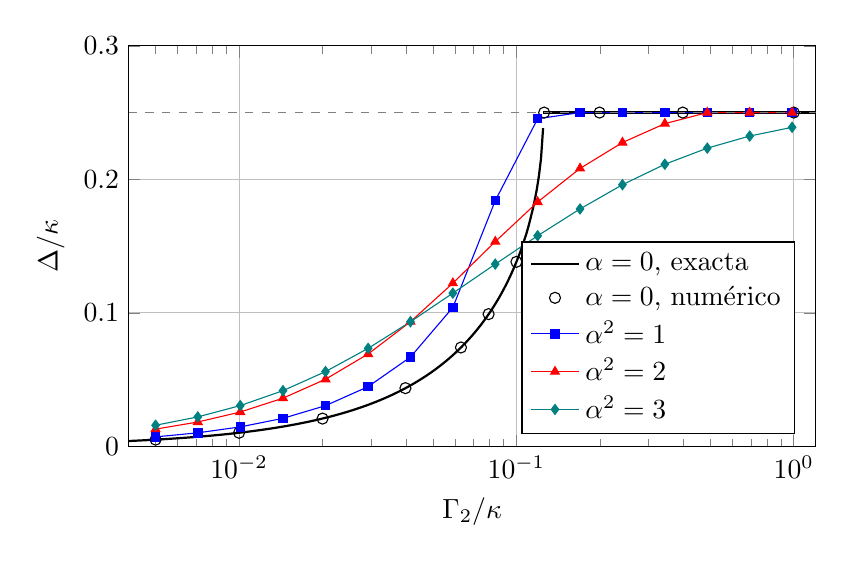
\begin{tikzpicture}
\begin{axis}[
  width=0.85\textwidth, height=0.55\textwidth,
  xmode=log, xmin=0.004, xmax=1.2, ymin=0, ymax=0.3,
  xlabel={$\Gamma_{2}/\kappa$}, ylabel={$\Delta/\kappa$},
  legend pos=south east, legend cell align=left, grid=major]
\addplot[black, thick, domain=0.004:0.125, samples=200] {0.25*(1-sqrt(1-8*x))};
\addlegendentry{$\alpha=0$, exacta}
\addplot[black, thick, forget plot, domain=0.125:1.2] {0.25};
\addplot[only marks, mark=o, black] coordinates {
(0.0050,0.00506) (0.0100,0.01021) (0.0200,0.02082) (0.0398,0.04362)
(0.0631,0.07407) (0.0794,0.09906) (0.1000,0.13820) (0.1259,0.25)
(0.1995,0.25) (0.3981,0.25) (1.0,0.25)};
\addlegendentry{$\alpha=0$, num\'erico}
\addplot[blue, mark=square*, mark size=1.5pt] coordinates {
(0.0050,0.00711) (0.0071,0.01017) (0.0101,0.01459) (0.0144,0.02103)
(0.0205,0.03051) (0.0292,0.04475) (0.0415,0.06690) (0.0590,0.10407)
(0.0839,0.18404) (0.1193,0.24538) (0.1696,0.25) (0.2412,0.25)
(0.3430,0.25) (0.4878,0.25) (0.6937,0.25) (0.9865,0.25)};
\addlegendentry{$\alpha^{2}=1$}
\addplot[red, mark=triangle*, mark size=1.8pt] coordinates {
(0.0050,0.01292) (0.0071,0.01826) (0.0101,0.02574) (0.0144,0.03611)
(0.0205,0.05029) (0.0292,0.06921) (0.0415,0.09338) (0.0590,0.12223)
(0.0839,0.15335) (0.1193,0.18303) (0.1696,0.20815) (0.2412,0.22755)
(0.3430,0.24171) (0.4878,0.25) (0.6937,0.25) (0.9865,0.25)};
\addlegendentry{$\alpha^{2}=2$}
\addplot[teal, mark=diamond*, mark size=1.8pt] coordinates {
(0.0050,0.01583) (0.0071,0.02209) (0.0101,0.03055) (0.0144,0.04174)
(0.0205,0.05603) (0.0292,0.07342) (0.0415,0.09335) (0.0590,0.11476)
(0.0839,0.13651) (0.1193,0.15775) (0.1696,0.17783) (0.2412,0.19597)
(0.3430,0.21130) (0.4878,0.22338) (0.6937,0.23242) (0.9865,0.23897)};
\addlegendentry{$\alpha^{2}=3$}
\addplot[gray, dashed, domain=0.004:1.2] {0.25};
\end{axis}
\end{tikzpicture}
\caption{Brecha de Liouville del modelo m\'inimo. La l\'inea negra es la soluci\'on exacta para $\alpha=0$ con el punto excepcional en $\Gamma_{2}=\kappa/8$; la l\'inea gris discontinua es el techo $\kappa/4$.}
\label{fig:gap}
\end{figure}

Se observan tres cosas:
\begin{enumerate}
\item Para $\GG$ peque\~no, la brecha coincide con la del modelo adiab\'atico $\GG\mathcal{D}[a^{2}-\alpha^{2}]$. Por ejemplo, con $\alpha^{2}=2$ y $\GG=0.005\kappa$ el modelo de dos niveles da $0.01292\kappa$ y el adiab\'atico $0.01283\kappa$.
\item En todos los casos la brecha satura en $\kappa/4$ y nunca lo supera, en acuerdo con el argumento de la Secci\'on 3.3.
\item El quiebre abrupto del punto excepcional solo aparece para $\alpha$ peque\~no. Para $\alpha^{2}\geq2$, el t\'ermino $-G\alpha^{2}(\spl+\smi)$ acopla bloques con distinto $\hat N$ y el punto excepcional se convierte en un cruce suave. Para $\alpha^{2}=2$ la parte imaginaria del modo lento solo aparece para $\GG\gtrsim0.5\kappa$, lejos de $\kappa/8$.
\end{enumerate}
Una estimaci\'on del cruce entre ambos reg\'imenes se obtiene igualando la brecha adiab\'atica al techo, $c(\alpha^{2})\GG^{\times}=\kappa/4$, lo que da $\GG^{\times}\approx0.18\kappa$, $0.10\kappa$ y $0.08\kappa$ para $\alpha^{2}=1,2,3$.

\subsection{Prueba con otros ingredientes}

Para ver si la desinton\'ia del qubit o la del modo generan un m\'aximo, se agregaron por separado $\Delta_{q}\spl\smi$ con $\Delta_{q}=0.144\kappa$ y $\delta_{m}a^{\dagger}a$ con $\delta_{m}=0.048\kappa$, los valores de la resonancia vestida, con $\alpha^{2}=2$. En ambos casos la brecha sigue creciendo mon\'otonamente hacia un valor cercano a $0.23\kappa$ en $\GG=\kappa$, sin m\'aximo. El t\'ermino $\delta_{m}a^{\dagger}a$ rompe adem\'as el espacio oscuro y crea un modo lento adicional, del orden de $10^{-3}\kappa$, que corresponde a relajaci\'on dentro del espacio del c\'odigo y no a la brecha de confinamiento.

\section{Comparaci\'on con el modelo completo y conclusiones}

\subsection{Qu\'e explica la derivaci\'on}

\begin{enumerate}
\item El mecanismo de saturaci\'on queda explicado de forma exacta: la brecha es la tasa de decaimiento de coherencias entre el espacio oscuro y estados vestidos qubit-pares, y esa tasa est\'a acotada por $\kappa/2$ multiplicado por el peso del qubit excitado, que en acoplamiento fuerte es $1/2$. De ah\'i el techo $\kappa/4$.
\item Para $\alpha=0$, la transici\'on es un punto excepcional en $\GG=\kappa/8=0.125\kappa$, en el mismo valor que se hab\'ia identificado. Pero para gatos de tama\~no \'util, $\alpha^{2}\geq2$, se convierte en un cruce suave.
\item El techo $\kappa/4$ es el mismo que aparece en la brecha de enganche semicl\'asica para un buffer arm\'onico, $\Delta_{\mathrm{lock}}\sim\min(4g_{2}^{2}\alpha^{2}/\kappa_{b},\,\kappa_{b}/4)$ \cite{Ferrari2026}. En este nivel, el buffer de dos niveles no se distingue del arm\'onico.
\end{enumerate}

\subsection{Qu\'e no explica}

El modelo completo muestra dos rasgos que el modelo m\'inimo no reproduce:
\begin{enumerate}
\item Un m\'aximo en $\Gamma_{2}^{-}/\kappa\approx0.13$ seguido de un descenso. En el modelo m\'inimo la brecha es mon\'otona: crece y satura, nunca decrece.
\item Un valor de saturaci\'on entre $0.10\kappa$ y $0.17\kappa$, claramente por debajo de $\kappa/4$.
\end{enumerate}
La coincidencia num\'erica entre el m\'aximo del modelo completo y $\kappa/8$ es, con lo derivado aqu\'i, probablemente accidental: para $\alpha^{2}=2$ el modelo m\'inimo no tiene ning\'un rasgo especial en $\GG=\kappa/8$.

\subsection{Veredicto}

La hip\'otesis de que el m\'aximo de la brecha es un punto excepcional del intercambio qubit-pares no se sostiene en su forma original. Lo que s\'i queda establecido es un resultado exacto para $\alpha=0$, el techo $\kappa/4$ y el cruce suave para gatos de tama\~no \'util. Pero ese resultado es, en lo esencial, el an\'alogo para un auxiliar de dos niveles de lo ya conocido para buffers arm\'onicos.

El m\'aximo y la saturaci\'on por debajo de $\kappa/4$ en el modelo completo deben venir de ingredientes que el modelo m\'inimo omite. Los candidatos son: los canales de un fon\'on $\Gamma_{1}^{\pm}$, el Kerr $\delta_{k}$, los t\'erminos no resonantes de la transformaci\'on polar\'onica y la dependencia temporal que captura el propagador de Floquet. Tambi\'en hay que descartar que la definici\'on de brecha usada en las tareas num\'ericas (la brecha robusta) mida un modo distinto del que se estudia aqu\'i. Identificar cu\'al de ellos produce el m\'aximo requiere validaci\'on computacional antes de cualquier derivaci\'on adicional.

\bibliographystyle{unsrt}
\bibliography{refs}

\end{document}
